% !TEX TS-program = pdflatex
% !TEX encoding = UTF-8 Unicode

% This is a simple template for a LaTeX document using the "article"
% class.  See "book", "report", "letter" for other types of document.

\documentclass[11pt]{article} % use larger type; default would be 10pt

%\usepackage[utf8]{inputenc} % set input encoding (not needed with
%XeLaTeX)


%%% Examples of Article customizations
% These packages are optional, depending whether you want the features
% they provide.  See the LaTeX Companion or other references for full
% information.

%%% PAGE DIMENSIONS
\usepackage{geometry} % to change the page dimensions
\geometry{a4paper} % or letterpaper (US) ocher a5paper or....
\geometry{margin=1in} % for example, change the margins to 2 inches
                      % all round
% \geometry{landscape} % set up the page for landscape
%   read geometry.pdf for detailed page layout information

\usepackage{graphicx} 
% \usepackage[parfill]{parskip} % Activate to begin paragraphs with an
% empty line rather than an indent

%%% PACKAGES
%\usepackage{booktabs} % for much better looking tables
\usepackage{array} % for better arrays (eg matrices) in maths
%\usepackage{paralist} % very flexible & customisable lists
%(eg. enumerate/itemize, etc.)
\usepackage{verbatim} % adds environment for commenting out blocks of
                      % text & for better verbatim
%\usepackage{subfig} % make it possible to include more than one
%captioned figure/table in a single float
% These packages are all incorporated in the memoir class to one
% degree or another...

%%% HEADERS & FOOTERS
\usepackage{fancyhdr} % This should be set AFTER setting up the page
                      % geometry
\pagestyle{fancy} % options: empty , plain , fancy
\renewcommand{\headrulewidth}{0pt} % customise the layout...
\lhead{}\chead{}\rhead{}
\lfoot{}\cfoot{\thepage}\rfoot{}

%%% SECTION TITLE APPEARANCE
%\usepackage{sectsty}
%\allsectionsfont{\sffamily\mdseries\upshape} % (See the fntguide.pdf
%for font help)

% (This matches ConTeXt defaults)

%%% ToC (table of contents) APPEARANCE
%\usepackage[nottoc,notlof,notlot]{tocbibind} % Put the bibliography
%in the ToC \usepackage[titles,subfigure]{tocloft} % Alter the style
%of the Table of Contents
%\renewcommand{\cftsecfont}{\rmfamily\mdseries\upshape}
%\renewcommand{\cftsecpagefont}{\rmfamily\mdseries\upshape} % No bold!

%\usepackage[T1]{fontenc}
\usepackage[latin9]{inputenc}
%\usepackage[active]{srcltx}
\usepackage{setspace}
\usepackage{lscape}
\doublespacing
\usepackage[english]{babel}
\bibliographystyle{naturemag}
\begin{document}

\title{SI:  Approaches for Large Scale Metagenome Assembly}
\author{ACH, JMT, CTB}
\maketitle

\subsubsection{Summary of approaches used on mock community dataset}

The HMP mock community dataset and its available draft reference
genomes were used to evaluate our approaches towards data reduction
and partitioning for \emph{de novo} metagenomic assembly.  Reads of
the mock community dataset were initially digitally normalized to a
coverage threshold of 20 (as previously described in \cite{browndiginorm}),
reducing the total number of reads from 14 to 11 million.
Additionally, to remove possible sequencing artifacts associated with
high coverage sequences (previously described in Howe et al., in preparation),
highly-abundant sequences (20-mers present at coverage greater than
50-fold) were filtered and the dataset was further normalized to a
coverage of 10, resulting in a total of 9 million reads (Fig.
3).  Finally, the remaining reads were divided into
disconnected sets of reads resulting in a total of 85,818 partitions
containing greater than five reads (summarized in
Table 1).

\section{Methods}

\subsection{Datasets}
In this study, we examined two large soil metagenomes generated from
soils collected from Iowa corn and native prairie soils.  Sequencing
was performed at the DOE Joint Genome Institute (Walnut Creek, CA).
Reads were quality trimmed at where Phred scores indicated a score of
'2'.  The total quality-trimmed reads in the Iowa corn and prairie
datasets were 1.8 million and 3.3 million, respectively.  We also
include a human gut mock community dataset (combined from SRA
SRX055381 and SRX055380).  For this mock community dataset, DNA from
bacterial isolates originally recovered from within or on the human
body was mixed together at staggered concentrations (over 5 orders of
magnitude based on genomic DNA concentrations) and sequenced.  The
mock community dataset originally contained 14.5 million reads.

To evaluate our approaches, we added simulated reads from either a
single E. Coli (str. K-12 substr DH10B) or five E. coli strains (K-12
substr DH10B, E24377, O147:H7 str. EC4115, UMN026, SE15) into select
metagenomes.  We computationally generated 100 bp reads from each
reference genome to a coverage of 10x and with a 2\% error rate and
subsequently randomly shuffled these reads with select datasets.

\subsubsection{Estimation of assembly requirements for soil metagenomes}
Subsets of the Iowa corn metagenome were assembled with the Velvet
assembler (v1.2.07) with the following parameters: velveth K=45,
-short and velvetg -exp\_cov auto -cov\_cutoff auto, -scaffolding no.
The time and memory for each assembly was estimated up to a maximum of
150 hours and 100 GB.

\subsubsection{Digital normalization}
Digital normalization was previously describe in \cite{browndiginorm}.  
For the mock
community dataset, digital normalization was performed with the
following parameters: K=20, coverage=20, and Bloom filter size = 1 GB
x 4.  For Iowa corn metagenome, digital normalization parameters were
as follows: K=20, coverage=20, and Bloom filter size = 48 GB x 4.
Similar parameters were used for the Iowa prairie metagenome, with the
exception that the Bloom filter size was 60 GB x 4.

\subsubsection{Removal of high abundance sequences}
To eliminate known sequencing artifacts in Illumina metagenomes
(previously described in Howe et al., in preparation), high abundance 
sequences (coverage
greater than 50) were removed using the count-min-sketch datastructure
used for digital normalization.  For the relatively high coverage mock
community dataset, filtered reads were subsequently normalized to a
coverage of 10 (K=20, bloom filter size = 1 GB x 4).

\subsubsection{Partitioning and \emph{de novo} assembly of disconnected reads}
Normalized and filtered datasets were loaded into a probabilistic
representation of the assembly graph as described in \cite{Pell:2012cq}, and
disconnected partitions of the resulting graph were separated.
Partitions containing less than five reads were discarded.  Each
partition was subsequently assembled using the Velvet assembler with
the same setting as described above, with the exception that K=35-59
and shortPaired setting was used for paired end reads.  The resulting
contigs greater than 300 bp from multiple-K assemblies were
dereplicated with CD-HIT (\cite{Fu:2012jk}, 99\% similarity) and merged with
Minimus2 \cite{Sommer:2007p1253}.


\subsection{Comparing coverage of reference genomes by reads}
Reads in the HMP mock unfiltered and filtered datasets were mapped
back to originating genomes using default settings in Bowtie2
\cite{bowtie}.  For cases where reads could be mapped back to multiple
genomes, a single genome was randomly selected to be identified with
each read.  Sequencing coverage was estimated for the whole genome as
the median base pair coverage for all base pairs in the reference
genome.

\subsection{Read coverage by assemblies}
All quality trimmed reads for Iowa corn and prairie were aligned with
assembled contigs (length greater than 300 bp) using default
parameters in Bowtie2 \cite{bowtie}.  Paired end reads were evaluated according to
concordance with paired end library preparation (i.e. paired end reads
on opposite DNA strands) and the alignment of both pairs of reads to
an assembled contig.  The base pair coverage of each contig was
estimated with the median base pair coverage of all reads across the
length of the contig.  Additionally, for each position in a contig
(with the exception of the external 100 bp on each end), the
percentage of the mapped consensus base pair was calculated.  The
fraction of positions with greater than 95\% base consensus was
calculated to estimate the presence of polymorphisms within the
assembled contig.

\subsection {Annotation of assemblies}
Assembled contigs and their corresponding median bp coverage for the
Iowa corn and prairie metagenomes were upload into MG-RAST annotation
pipeline \cite{Meyer:2008db} and are available on MG-RAST as 4504979.3 (Iowa corn)
and 4504798.3 (Iowa Prairie).  The resulting MG-RAST blat annotations
were compared to the M5NR database using a maximum e-value of 1e-5, a
minimum identity of 60\%, and a minimum alignment length of 15 aa.  The M5NR is an 
integration of numerous databases including protein annotations from GenBank, IMG, 
KEGG, PATRIC, RefSeq, SEED, SwissProt, and TrEMBL and ontology annotations from 
eggNOG, COG, GO, KO, NOG, and SEED subsystems. Both the phylogenetic 
distribution of bacteria (phyla) and functional
distribution of subsystems were compared between the Iowa and corn
metagenomes.
  
\subsection{Comparing assemblies}
Resulting assemblies (contigs greater than 300 bp) were compared using
the total number of contigs, assembly length, and maximum contig size
for each assembly.  Assemblies were also aligned to each other using
blastn and the resulting coverage of each assembly was calculated.  In
the case of the mock community, the resulting assemblies were also
aligned to sequenced draft genomes of the original isolates and, if
applicable, spiked reference genomes. Abundance of assembled contigs
and reference genomes were estimated by mapping raw reads with Bowtie
(allowing up to 2 mismatches for a match).  The median base pair
coverage was used to estimate abundances.  Associated assembled
contigs (greater than 300 bp) from the unfiltered and filtered
(digital normalized) assemblies were identified using a blastn
alignment (requiring E-value cutoff of 1e-5).  Contigs were associated
with reference genomes through an identical alignment approach.

The reference-based abundance (from reads mapped to reference genomes)
and assembly-based abundance (from reads mapped to contigs) of genomes
were compared.  Using a one-directional, paired t-test of squared
deviations, the abundance estimates of the unfiltered and filtered
assemblies were compared.  We expected the filtered assembly to have
increased accuracy due to a reduction of errors (e.g. normalization
and high abundance filtering) and used a one-sided t-test which
indicated that abundance estimations from the filtered assembly were
significantly closer to predicted abundances from reference genomes
(p-value of 0.032).

Annotations against the M5NR database were obtained through the
MG-RAST annotation pipeline (maximum E-value 1e-5, minimum identity 60\%, minimum alignment length 15 aa). The phylogenetic and functional
distribution of SEED subsystems between the Iowa corn and prairie
metagenome were compared (Fig. 6 and 7).  For each subsystem, the
relative abundance of each subsystem was calculated and the ratio of
the fraction present in the Iowa corn and prairie was determined
(e.g., the relative abundance of a subsystem which was equally
represented in both corn and prairie metagenomes would equal 1).  To
estimate similarity among all subsystems and phyla, the following was
calculated: ((1 - ratio)$^2$)$^{0.5}$ where a value closer to 0
indicates higher similarity.  Overall, for the phylogenetic and
functional distribution of SEED annotations, this value was 0.35 +/-
0.57 and 0.10 +/- 0.08.

%\subsection{Identification of \emph{gyrB}, \emph{recA}, and
%\emph{rplB}}

%Well-curated sequences from the Ribosomal Database Project's (RDP)
%Functional Gene Repository were used to build HMM profiles for
%\emph{gyrB}, \emph{recA}, and \emph{rplB}.  These models are
%available upon request from RDP.  The \emph{gyrB}, \emph{recA}, and
%\emph{rplB} HMM models contained 809, 353, and 277 amino acids,
%respectively.  Assembled contigs were translated in all six reading
%frames and searched against the HMM profiles using HMMER3 (v3.0).
%Results were filtered with an E-value threshold of 1e-3.  The
%abundance of assembled contigs were previously calculated as
%described above and used to estimate total number of \emph{gyrB},
%\emph{recA}, and \emph{rplB} genes within soil metagenomes.
%Benchmarking protein models against the HMP mock community with a
%known number of genomes, we found that recA and rplB best identified
%total genome count for the HMP mock dataset (Supp Table X) and
%subsequently used these two genes to estimate genome abundance within
%Iowa corn and prairie metagenomes.

\section{Supp. References}
\bibliography{assembly-paper}

\section{Figures and Tables}

\begin{landscape}
\begin{table}
\caption{HMP mock dataset reference genomes estimated sequencing depth
  (median bp coverage of reads), number of partitions, total length
  (bp), coverage of reference genomes by unfiltered reads (UF Cov),
  coverage of reference genomes by filtered reads (F Cov), coverage of
  reference genomes by unfiltered assembled contigs (UFA Cov), and
  coverage of reference genomes by filtered assembled contigs (FA
  Cov).}
\begin{tabular}{l c c c c c c c}
\hline Reference Genome & Coverage & No. Partitions & Length (bp) & UF
Cov (bp) & F Cov (bp) & UFA Cov & FA Cov \\ \hline
gi\textbar{}32470588\textbar{}ref\textbar{}NC\_005008.1\textbar{} &
2,412 & 9 & 4,439 & 4,439 & 1,058 & 100 \% & 28 \% \\
gi\textbar{}32470581\textbar{}ref\textbar{}NC\_005007.1\textbar{} &
549 & 16 & 4,679 & 4,679 & 4,585 & 100 \% & 77 \% \\
gi\textbar{}32470520\textbar{}ref\textbar{}NC\_005003.1\textbar{} &
533 & 21 & 6,585 & 6,585 & 6,441 & 100 \% & 64 \% \\
gi\textbar{}32470572\textbar{}ref\textbar{}NC\_005006.1\textbar{} &
253 & 2 & 8,007 & 8,004 & 7,953 & 100 \% & 100 \% \\
gi\textbar{}32470532\textbar{}ref\textbar{}NC\_005004.1\textbar{} &
112 & 52 & 24,365 & 24,358 & 24,291 & 100 \% & 83 \% \\
gi\textbar{}126640109\textbar{}ref\textbar{}NC\_009084.1\textbar{} &
85 & 3 & 11,302 & 11,295 & 11,270 & 100 \% & 100 \% \\
gi\textbar{}32470555\textbar{}ref\textbar{}NC\_005005.1\textbar{} & 74
& 12 & 17,261 & 17,202 & 17,180 & 100 \% & 100 \% \\
gi\textbar{}10957398\textbar{}ref\textbar{}NC\_000958.1\textbar{} & 71
& 73 & 177,466 & 177,261 & 174,614 & 100 \% & 95 \% \\
gi\textbar{}10957530\textbar{}ref\textbar{}NC\_000959.1\textbar{} & 52
& 37 & 45,704 & 44,974 & 43,557 & 100 \% & 92 \% \\
gi\textbar{}126640097\textbar{}ref\textbar{}NC\_009083.1\textbar{} &
48 & 2 & 13,408 & 13,405 & 13,383 & 100 \% & 100 \% \\
gi\textbar{}15807672\textbar{}ref\textbar{}NC\_001264.1\textbar{} & 40
& 63 & 412,348 & 410,970 & 403,553 & 100 \% & 99 \% \\
gi\textbar{}15805042\textbar{}ref\textbar{}NC\_001263.1\textbar{} & 32
& 546 & 2,648,638 & 2,634,512 & 2,589,566 & 100 \% & 99 \% \\
gi\textbar{}27466918\textbar{}ref\textbar{}NC\_004461.1\textbar{} & 30
& 476 & 2,499,279 & 2,498,081 & 2,492,248 & 100 \% & 98 \% \\
gi\textbar{}125654693\textbar{}ref\textbar{}NC\_009008.1\textbar{} &
29 & 14 & 37,100 & 36,585 & 33,250 & 94 \% & 96 \% \\
gi\textbar{}161508266\textbar{}ref\textbar{}NC\_010079.1\textbar{} &
29 & 442 & 2,872,915 & 2,298,758 & 2,157,196 & 100 \% & 92 \% \\
gi\textbar{}77404776\textbar{}ref\textbar{}NC\_007490.1\textbar{} & 27
& 27 & 100,828 & 99,385 & 93,550 & 100 \% & 96 \% \\
gi\textbar{}125654605\textbar{}ref\textbar{}NC\_009007.1\textbar{} &
24 & 92 & 114,045 & 108,526 & 97,860 & 100 \% & 96 \% \\
gi\textbar{}77404693\textbar{}ref\textbar{}NC\_007489.1\textbar{} & 18
& 12 & 105,284 & 102,212 & 96,169 & 100 \% & 99 \% \\
gi\textbar{}24378532\textbar{}ref\textbar{}NC\_004350.1\textbar{} & 16
& 131 & 2,030,921 & 2,029,376 & 2,025,544 & 100 \% & 99 \% \\
gi\textbar{}77404592\textbar{}ref\textbar{}NC\_007488.1\textbar{} & 13
& 30 & 114,178 & 103,351 & 93,637 & 100 \% & 99 \% \\
gi\textbar{}77461965\textbar{}ref\textbar{}NC\_007493.1\textbar{} & 13
& 628 & 3,188,609 & 2,919,441 & 2,681,855 & 100 \% & 99 \% \\
gi\textbar{}77464988\textbar{}ref\textbar{}NC\_007494.1\textbar{} & 13
& 262 & 943,016 & 862,781 & 788,626 & 100 \% & 98 \% \\
gi\textbar{}126640115\textbar{}ref\textbar{}NC\_009085.1\textbar{} &
11 & 683 & 3,976,747 & 3,939,190 & 3,936,208 & 99 \% & 99 \% \\
gi\textbar{}148642060\textbar{}ref\textbar{}NC\_009515.1\textbar{} & 9
& 552 & 1,853,160 & 1,828,231 & 1,826,639 & 99 \% & 98 \% \\
gi\textbar{}150002608\textbar{}ref\textbar{}NC\_009614.1\textbar{} & 7
& 7,751 & 5,163,189 & 4,899,622 & 4,896,808 & 81 \% & 82 \% \\
gi\textbar{}15644634\textbar{}ref\textbar{}NC\_000915.1\textbar{} & 6
& 2,888 & 1,667,867 & 1,581,502 & 1,581,024 & 78 \% & 79 \% \\
gi\textbar{}194172857\textbar{}ref\textbar{}NC\_003028.3\textbar{} & 6
& 4,123 & 2,160,842 & 2,047,832 & 2,037,347 & 78 \% & 78 \% \\
gi\textbar{}49175990\textbar{}ref\textbar{}NC\_000913.2\textbar{} & 6
& 5,913 & 4,639,675 & 4,080,605 & 4,074,119 & 84 \% & 85 \% \\
gi\textbar{}50841496\textbar{}ref\textbar{}NC\_006085.1\textbar{} & 6
& 6,459 & 2,560,265 & 2,169,547 & 2,169,056 & 59 \% & 64 \% \\
gi\textbar{}77358697\textbar{}ref\textbar{}NC\_003112.2\textbar{} & 4
& 9,269 & 2,272,360 & 1,655,023 & 1,626,301 & 28 \% & 33 \% \\
\end{tabular}
\label{ref-summary}
\end{table}
\end{landscape}

\begin{table}[ht]
\caption{Number of housekeeping genes identified in HMP mock community
  reference genomes and assembled (Velvet) contigs.}
\begin{tabular}{l c c}
Gene model & Counts in ref genomes & Counts in assembled contigs \\
\hline
gyrB & 21 & 55 \\
recA & 22 & 19 \\
rplB & 18 & 18 \\
rpoB & 18 & 84 \\
\end{tabular}
\end{table}

\begin{figure}[ht]
\center{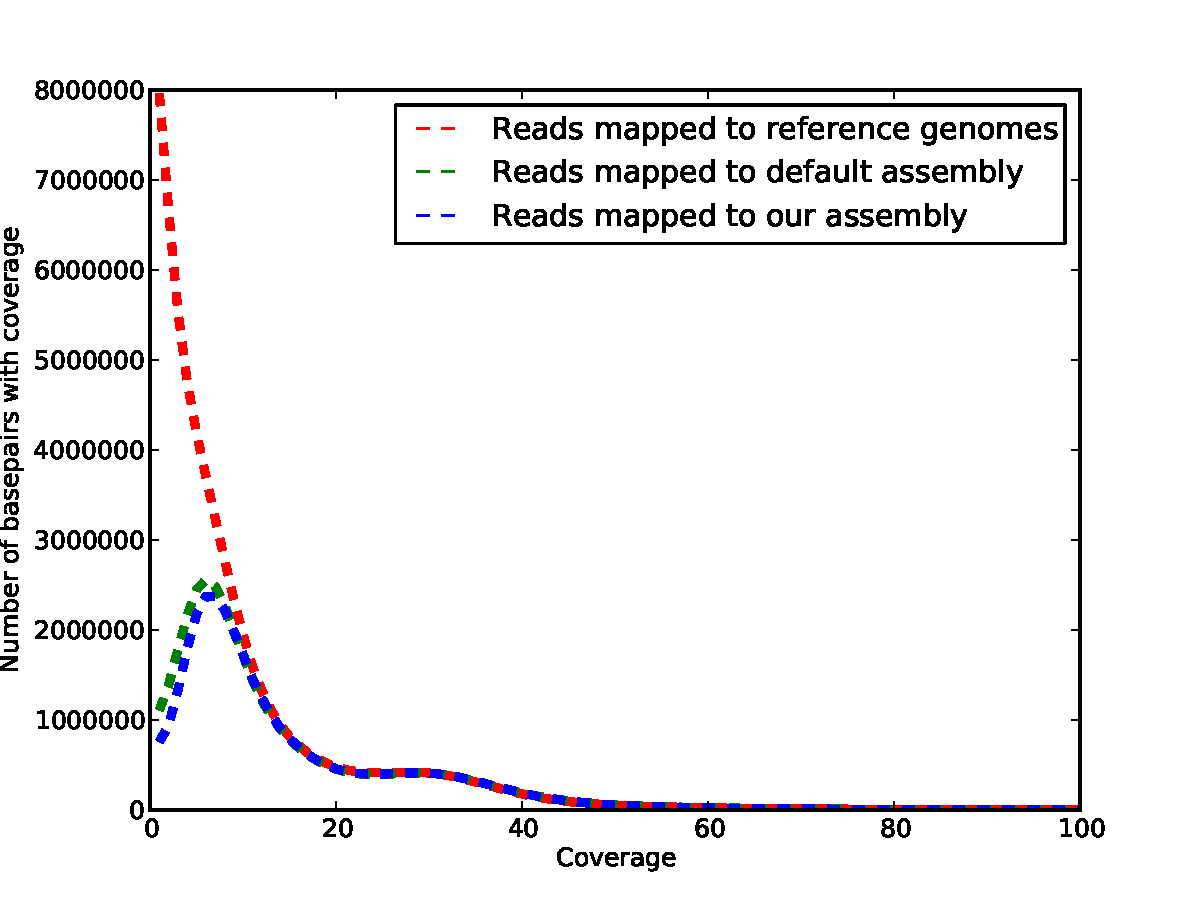
\includegraphics[width=\textwidth,height=\textheight,keepaspectratio]
{./figures/coverage.pdf}}
\caption{Number of basepairs with specified coverage for reads which
  map to reference genomes and unfiltered and filtered assembled
  contigs greater than 300 bp.}
\label{coveragehmp}
\end{figure}

\begin{figure}[ht]
\center{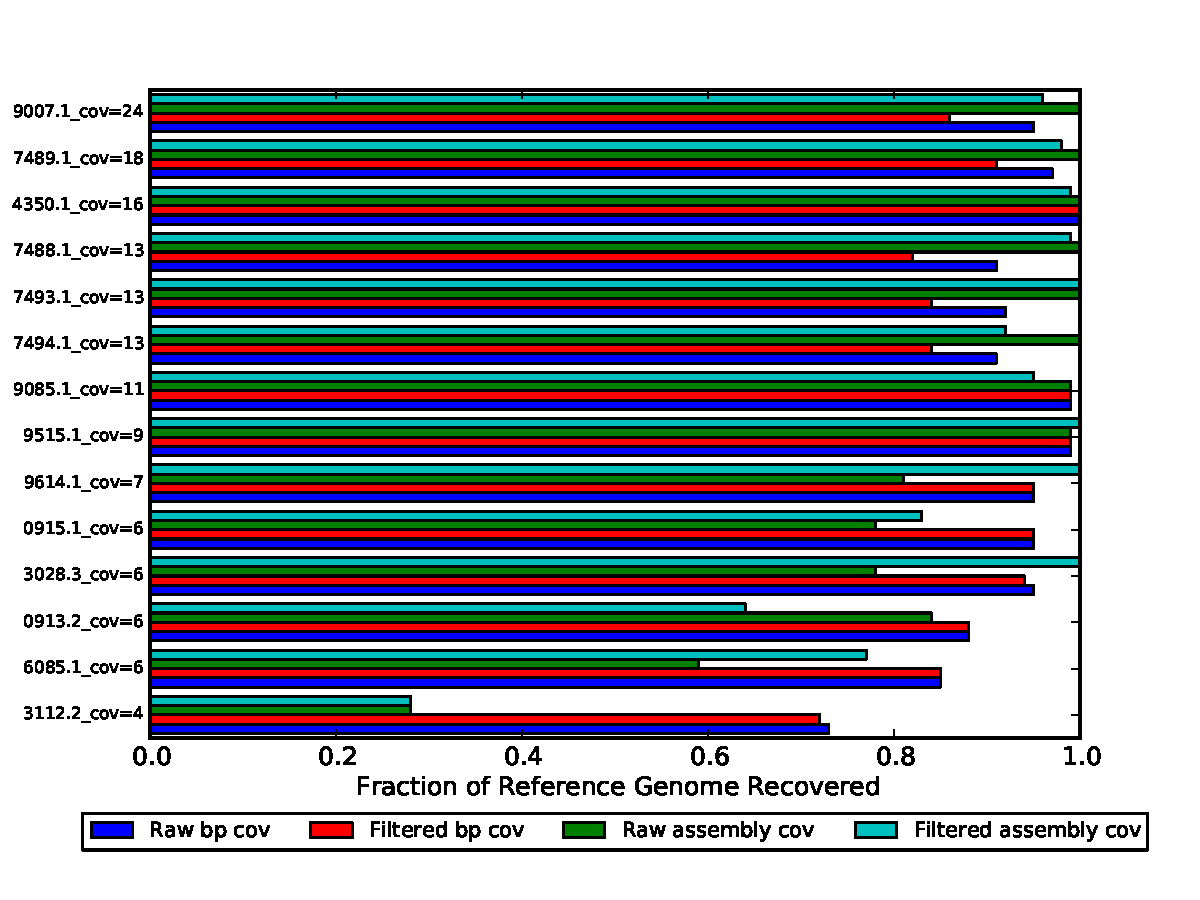
\includegraphics[scale=0.8]{./figures/coverage1.pdf}}
\caption{Coverage of reference genomes by unfiltered and filtered
  assembled contigs and unfiltered and filtered reads.}
\label{coverage1}
\end{figure}

\begin{figure}[ht]
\center{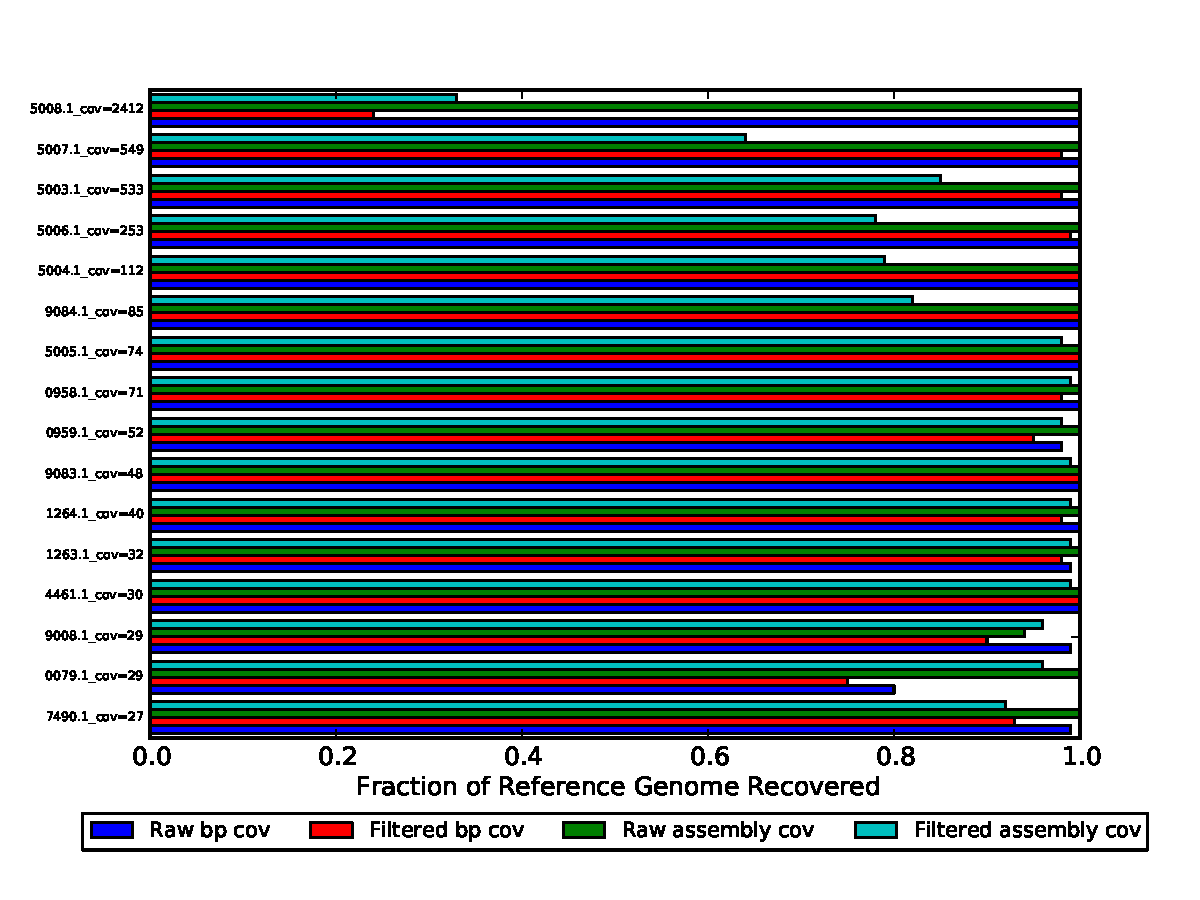
\includegraphics[scale=0.8]{./figures/coverage2.pdf}}
\caption{Coverage of reference genomes by unfiltered and filtered
  assembled contigs and unfiltered and filtered reads.}
\label{coverage2}
\end{figure}

\begin{figure}[ht]
\center{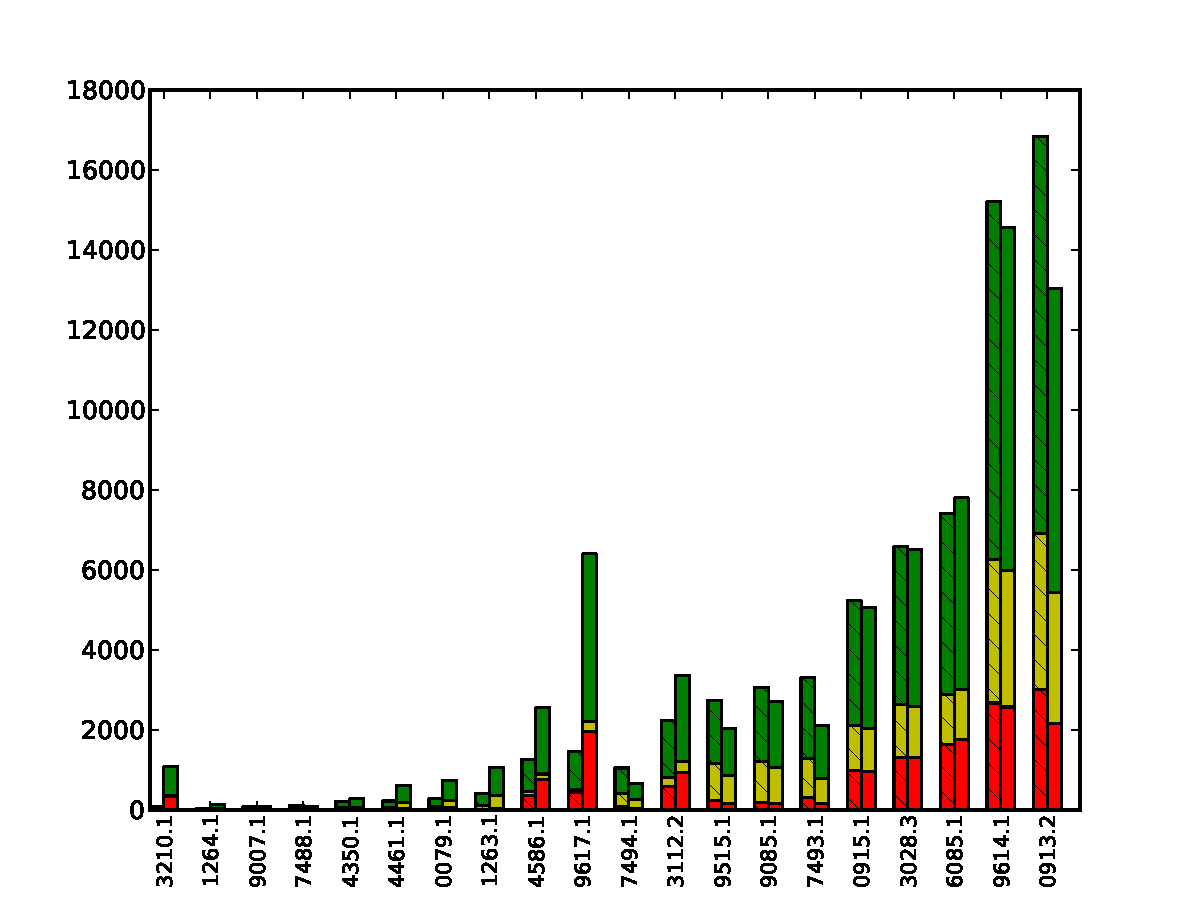
\includegraphics[scale=0.5]{./figures/contig-lengths.pdf}}
\caption{Total number of contigs for unfiltered (bars with hashed
  lines) and filtered (solid bars) for top twenty references with most
  assembled contigs (ranked by unfiltered assembly).  Red indicates
  contig lengths less than 500 bp, yellow indicates contig lengths
  between 500 bp and 3000 bp, and green indicates contig lengths
  greater than 5000 bp.  Reference genome IDs shown here are last 5
  digits of RefSeq ID.}
\label{contig-lengths}
\end{figure}

\begin{figure}[ht]
\center{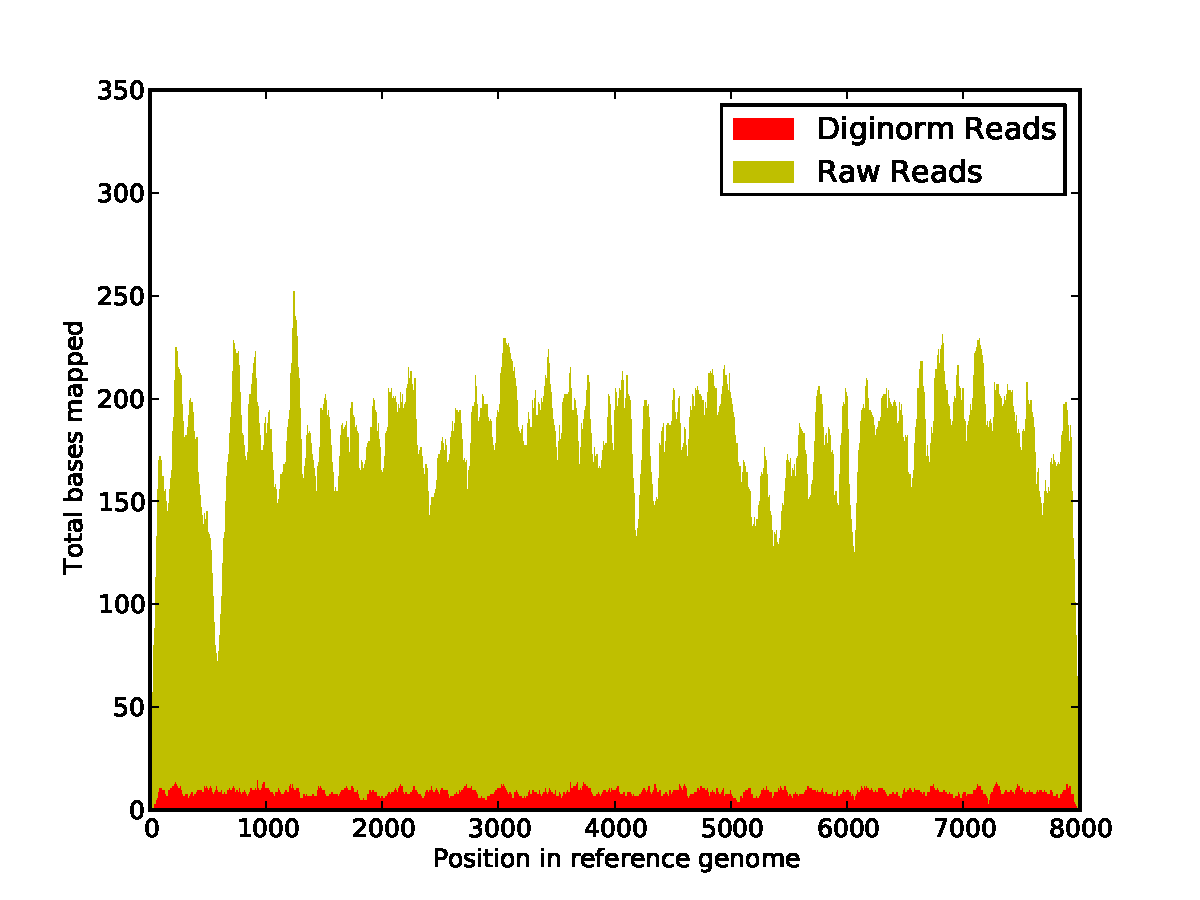
\includegraphics[width=\textwidth,height=\textheight,keepaspectratio]{./figures/ref_gi32470572.pdf}}
\caption{Alignment of reads (colored by originating partition) to
  reference genome NC\_00745901}
\label{diginormreference}
\end{figure}

\begin{figure}[ht]
\center{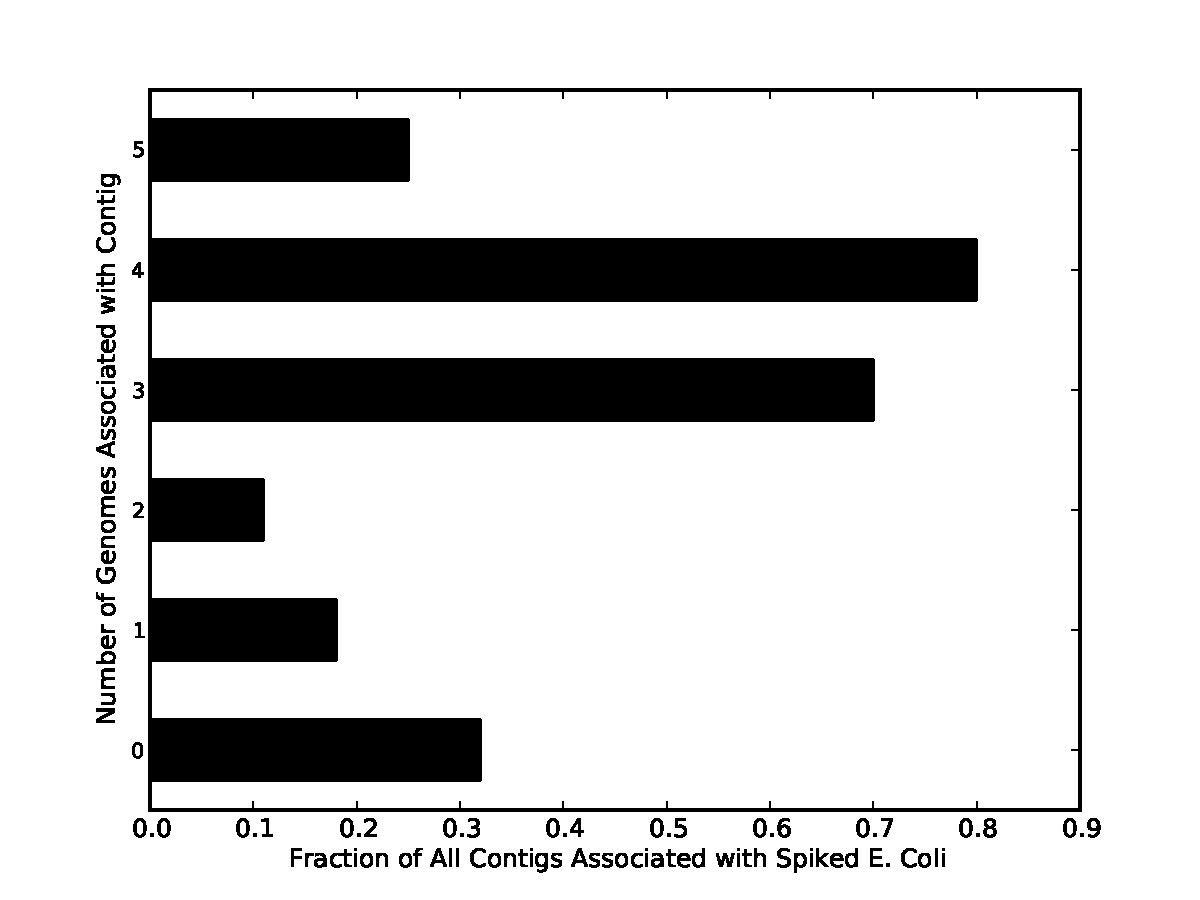
\includegraphics[width=\textwidth,height=\textheight,keepaspectratio]{./figures/ecoli-multi-genomes.pdf}}
\caption{The fraction of assembled contigs assembled from partitions
  containing spiked \emph{E. coli} reads associated with 0 to five of
  the \emph{E. coli} reference genomes.  The large majority of contigs
  contain reads associated with multiple genomes or to no genome.}
\label{fractionassembled}
\end{figure}



\begin{figure}[ht]
\center{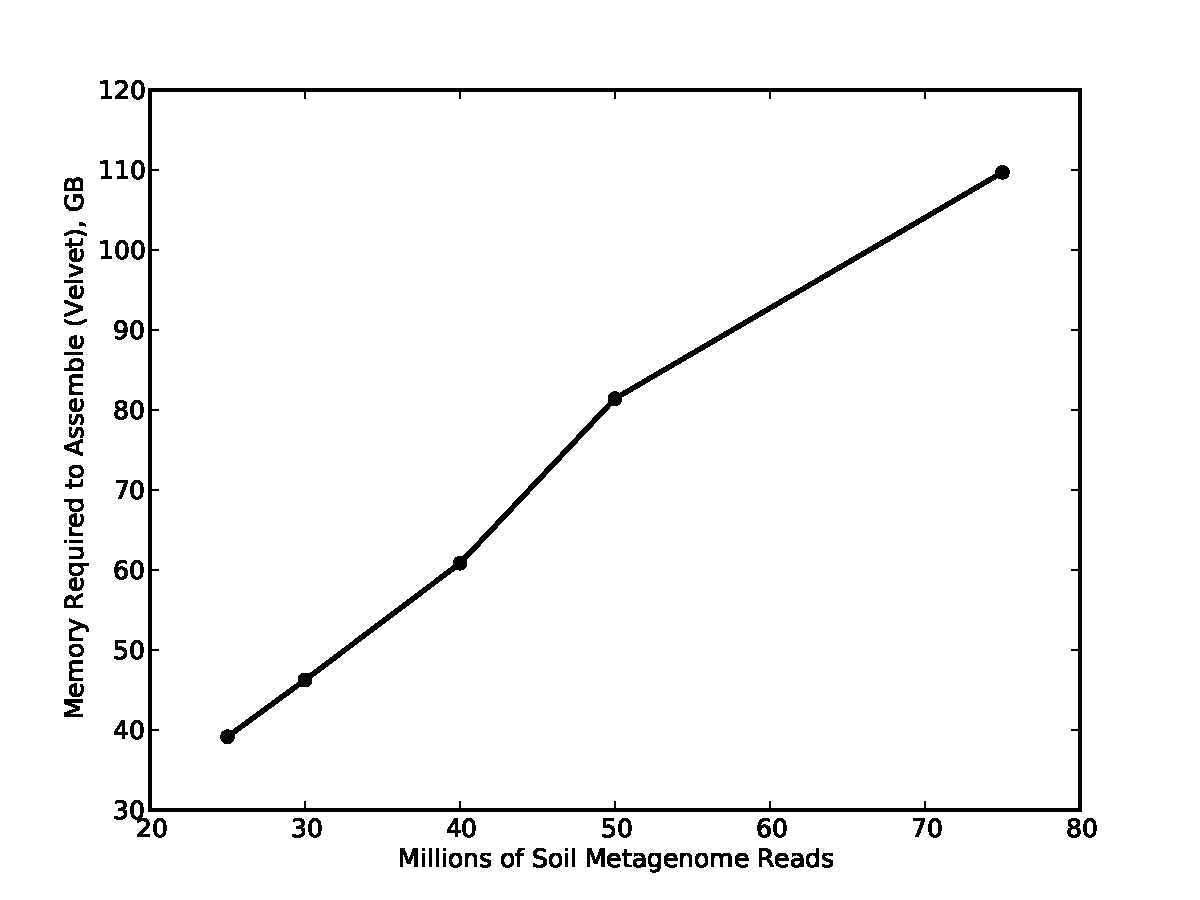
\includegraphics[width=\textwidth,height=\textheight,keepaspectratio]{./figures/memory.pdf}}
\caption{Memory requirements to assemble subsets of Iowa corn soil
  metagenome}
\label{memory}
\end{figure}

\begin{figure}[ht]
\center{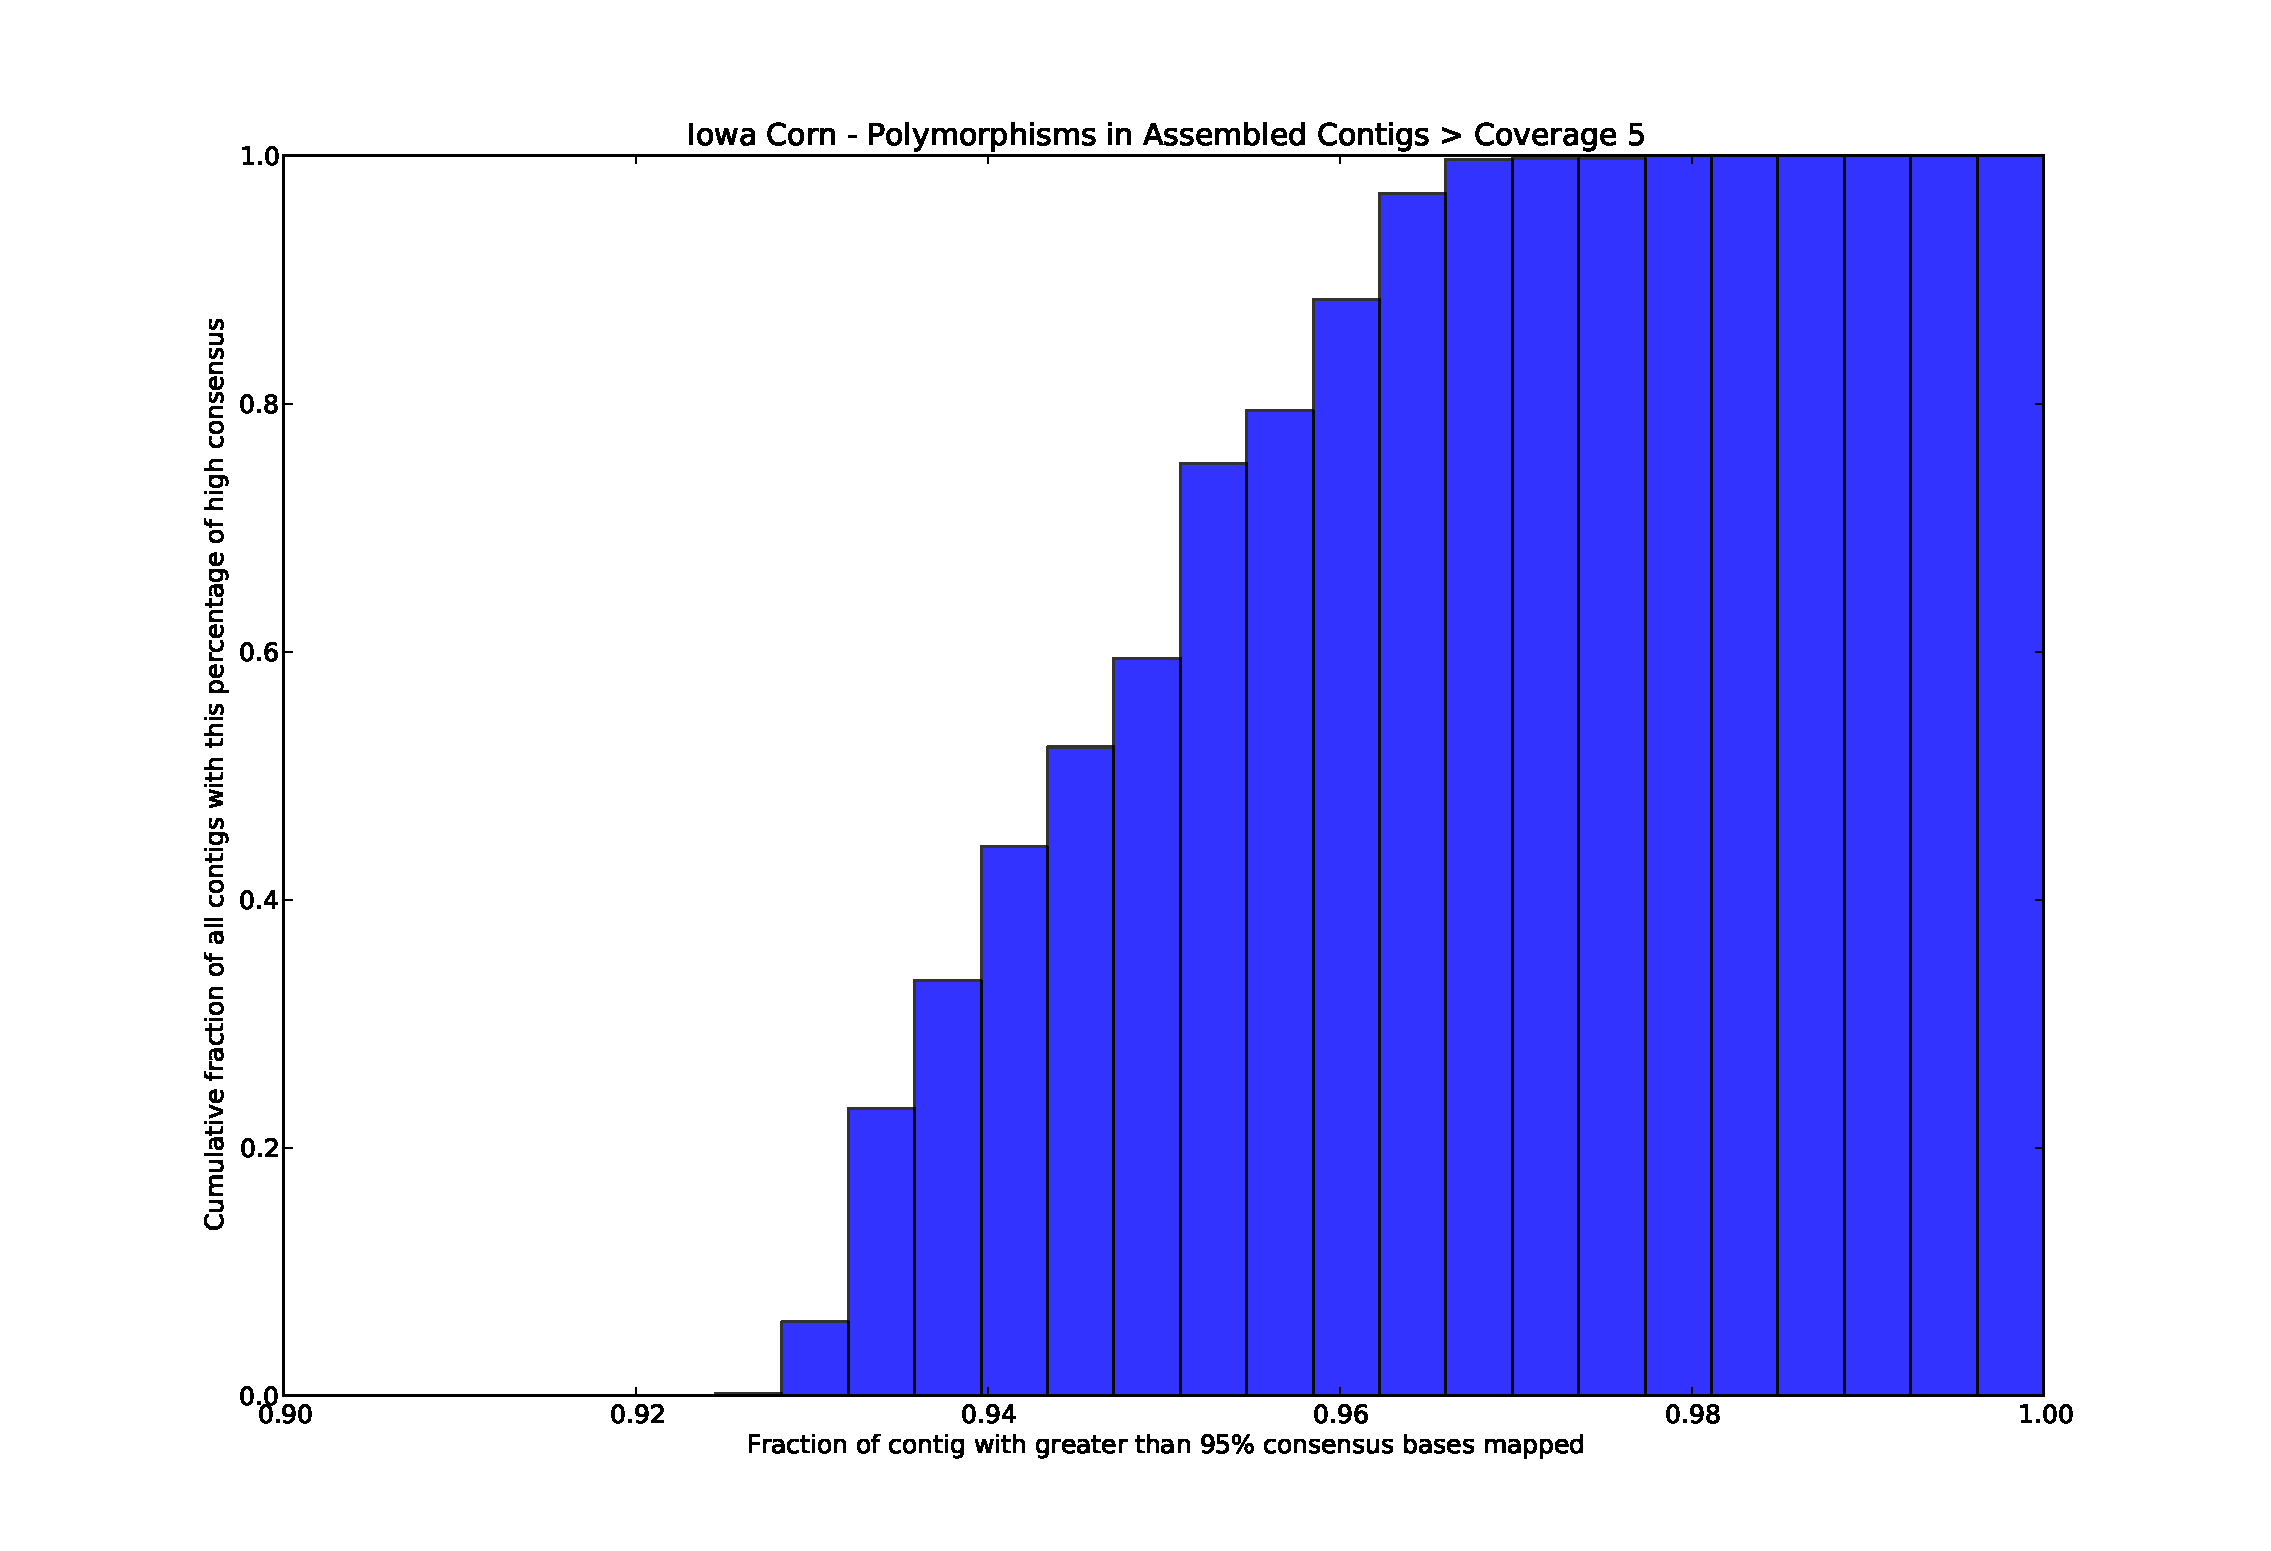
\includegraphics[width=\textwidth,height=\textheight,keepaspectratio]{./figures/corn.pdf}}
\caption{The presence of polymorphic sequences in assembled contigs of
  Iowa corn metagenome.}
\label{corn-poly}
\end{figure}

\begin{figure}[ht]
\center{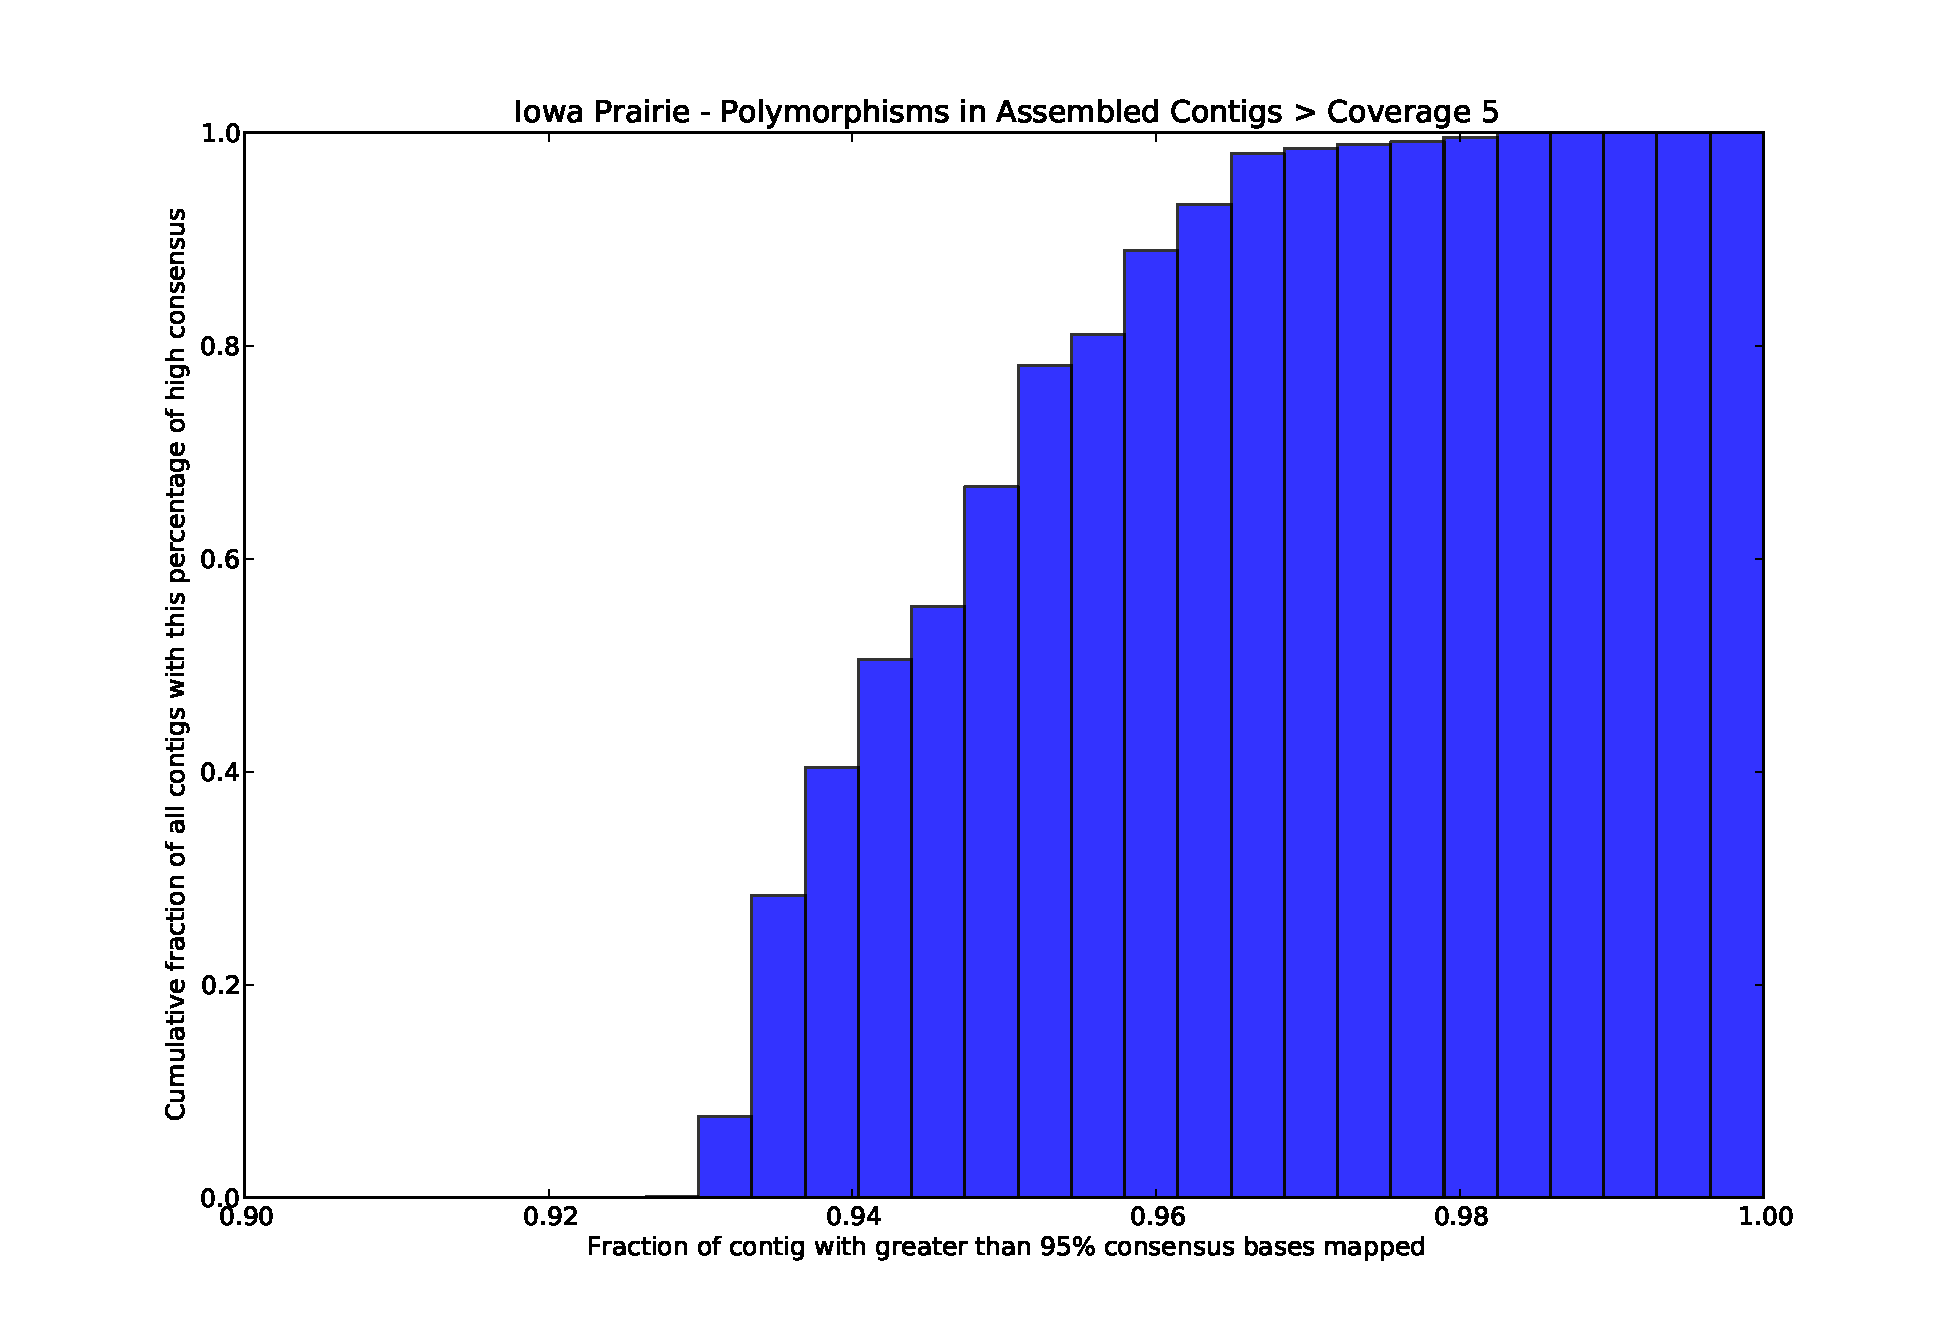
\includegraphics[width=\textwidth,height=\textheight,keepaspectratio]{./figures/prairie.pdf}}
\caption{The presence of polymorphic sequences in assembled contigs of
  Iowa prairie metagenome.}
\label{prairie-poly}
\end{figure}

\end{document}

